\chapter{Bacteriologia: crescimento, fisiologia e genética}\label{ch:b3:bacteriology}

Uma única célula de \emph{Escherichia coli} em caldo morno se divide a
cada vinte minutos. Se nada a detivesse, seus descendentes pesariam
mais que a Terra em dois dias; de fato eles param em poucas horas,
quando o açúcar acaba, e ficam por semanas num estado que sobrevive à
inanição. Uma bactéria aparentada, dados um ferimento e algumas horas,
torna-se cem milhões de células e uma febre; cem anos atrás ela matava
um terço dos pacientes que infectava, e desde 1941 o veneno de um mofo
contra ela salvou mais vidas que qualquer outro fármaco --- enquanto as
bactérias, nesses mesmos oitenta anos, evoluíram maneiras de contornar
cada \omterm{def:b3:bacteriology:antibiotics}{antibiótico} já feito. As bactérias foram os organismos em que se
mostrou pela primeira vez que os genes são DNA, em que a regulação
gênica foi compreendida primeiro, e de que se tiraram as ferramentas do
\cref{ch:b3:genetic-engineering}. Este capítulo as trata como
organismos: seu envoltório, a aritmética de seu crescimento num frasco
e numa cultura contínua, o modo como uma população percebe sua própria
densidade, o tráfego de genes entre células, e a química e a evolução
dos \omterm{def:b3:bacteriology:antibiotics}{antibióticos} e da resistência.

\section{A célula bacteriana}

\begin{definition}[O envoltório]\label{def:b3:bacteriology:envelope}
\index{peptidoglicano}\index{Gram-positiva}\index{Gram-negativa}\index{membrana externa}\index{lipopolissacarídeo}\index{endósporo}
Toda bactéria, salvo umas poucas, é envolvida por uma parede de
\emph{peptidoglicano}: cadeias alternadas de N-acetilglicosamina e
ácido N-acetilmurâmico, com ligações cruzadas de peptídeos curtos que
as unem numa única molécula, a qual cerca a célula e resiste à pressão
de turgor --- de várias atmosferas --- do citoplasma. As bactérias
\emph{Gram-positivas} têm uma parede espessa de
\qtyrange{20}{80}{nm}, de muitas camadas, entremeada de ácidos
teicoicos; as \emph{Gram-negativas} têm uma parede fina de uma ou duas
camadas e, fora dela, uma segunda bicamada lipídica, a \emph{membrana
externa}, cuja monocamada externa é \emph{lipopolissacarídeo} (LPS, a
endotoxina --- a molécula que o sistema imune inato do
\cref{ch:b3:innate-immunity} reconhece e que causa o choque séptico), e
que fecha um periplasma. Porinas na membrana externa deixam entrar
moléculas pequenas e barram muitos \omterm{def:b3:bacteriology:antibiotics}{antibióticos}. Por fora pode haver
uma cápsula de polissacarídeo contra os fagócitos, flagelos para nadar
(\cref{ch:b3:cytoskeleton-motility}) e pili para adesão e \omterm{def:b3:bacteriology:hgt}{conjugação}.
Por dentro, o cromossomo --- uma molécula circular de
\qtyrange{1}{10}{Mb} na maioria das espécies --- é dobrado num
nucleoide sem membrana, ao lado dos \omterm{def:b3:genetic-engineering:tools}{plasmídeos}. Alguns gêneros
(\emph{Bacillus}, \emph{Clostridium}) conseguem encerrar uma cópia do
cromossomo num revestimento espesso como \emph{endósporo}, desidratado
e metabolicamente inerte, que sobrevive à fervura, à radiação e a
séculos de seca e germina quando os nutrientes voltam.
\end{definition}

\begin{method}[A coloração de Gram]\label{met:b3:bacteriology:gram}
\index{coloração de Gram}
O teste mais antigo do laboratório de bacteriologia (Gram, 1884) ainda
decide a primeira escolha de \omterm{def:b3:bacteriology:antibiotics}{antibiótico}. (1) Faça um esfregaço da
amostra e fixe-o pelo calor; (2) core com cristal violeta e depois com
iodo, que forma com o corante um grande complexo insolúvel dentro das
células; (3) lave com álcool: o \omterm{def:b3:bacteriology:envelope}{peptidoglicano} espesso das
\omterm{def:b3:bacteriology:envelope}{Gram-positivas}, desidratado pelo álcool, aprisiona o complexo e as
células ficam roxas, ao passo que a parede fina das \omterm{def:b3:bacteriology:envelope}{Gram-negativas} o
deixa sair; (4) contracore com safranina, que tinge de rosa as
\omterm{def:b3:bacteriology:envelope}{Gram-negativas} agora incolores. A forma e o arranjo --- cocos em cachos
(estafilococos) ou em cadeias (estreptococos), bastonetes, espirais ---
estreitam ainda mais a identificação, e um coco roxo em cachos vindo de
um abscesso é um estafilococo antes que qualquer cultura tenha
crescido.
\end{method}

\begin{omfigure}
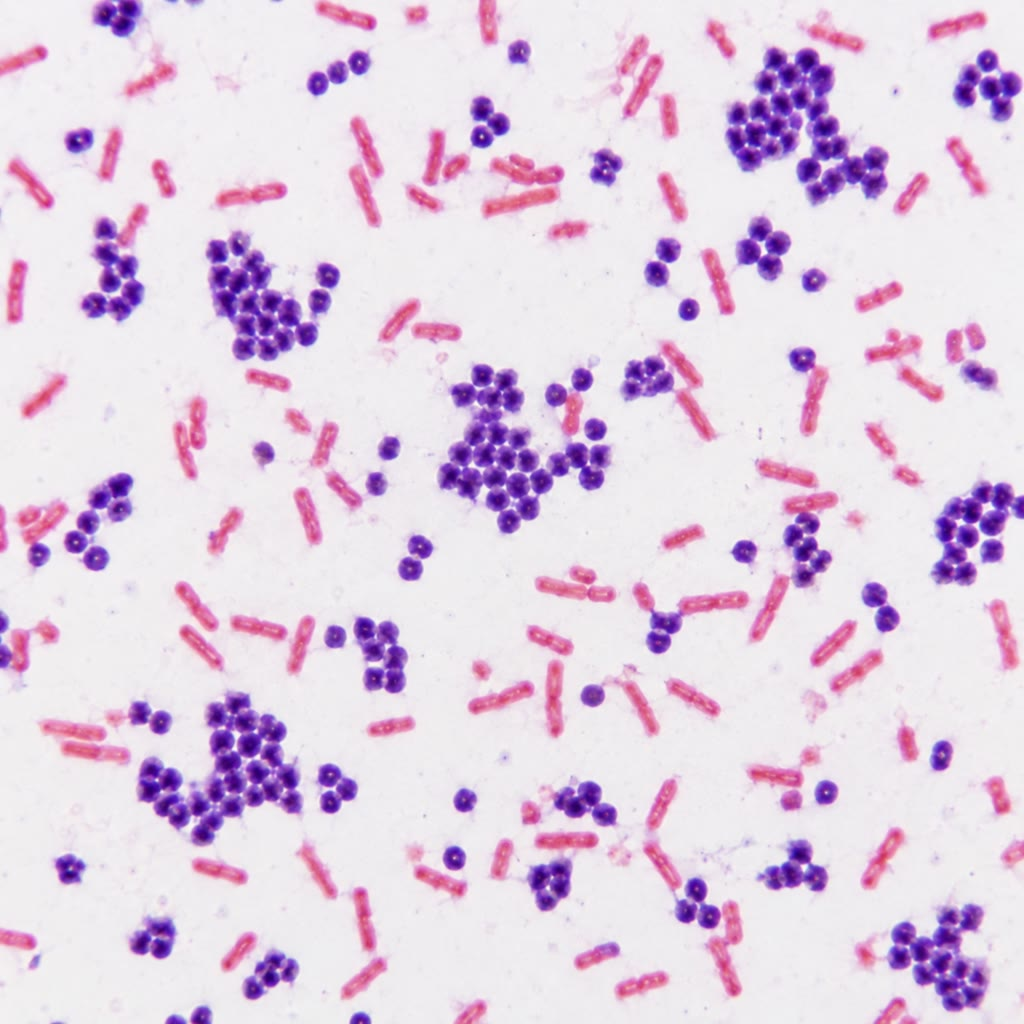
\includegraphics[width=0.36\linewidth]{images/book5/ai/b5-12-gram-stain.jpg}\hspace{0.04\linewidth}
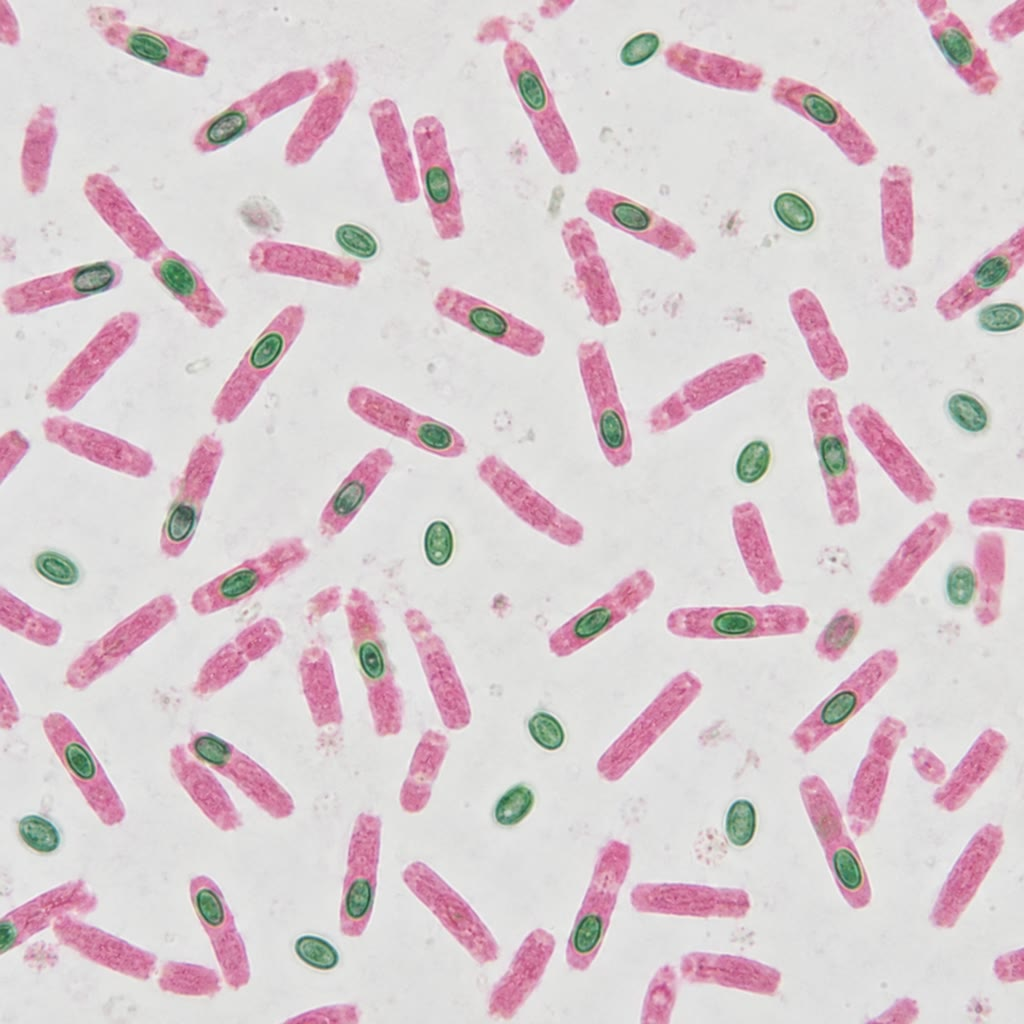
\includegraphics[width=0.36\linewidth]{images/book5/ai/b5-12-endospores.jpg}

{\small À esquerda: uma \omterm{met:b3:bacteriology:gram}{coloração de Gram} --- cocos Gram-positivos roxos
em cachos, bastonetes Gram-negativos rosados. À direita: células de
\emph{Bacillus} coradas para \omterm{def:b3:bacteriology:envelope}{endósporos}, os ovais verde-brilhantes
dentro de células rosadas e esporos livres ao lado delas.}
\end{omfigure}

\begin{omfigure}
\begin{tikzpicture}[every node/.style={font=\scriptsize}, >=stealth]
  % Gram-positive
  \begin{scope}
    \fill[omDef!15] (0,0) rectangle (4.5,0.4); \draw[thick, omDef] (0,0) -- (4.5,0); \draw[thick, omDef] (0,0.4) -- (4.5,0.4);
    \fill[omProp!40] (0,0.5) rectangle (4.5,2.0); \foreach \y in {0.7,0.95,1.2,1.45,1.7} \draw[omProp!80!black, thin] (0,\y) -- (4.5,\y);
    \foreach \x in {0.6,1.6,2.6,3.6} \draw[omMeth!70!black, thick] (\x,0.5) -- (\x,2.3);
    \node[below] at (2.25,-0.1) {membrana citoplasmática};
    \node[right, align=left] at (4.6,1.25) {peptidoglicano espesso\\(\qtyrange{20}{80}{nm})}; \node[right, omMeth!70!black] at (4.6,2.2) {ácidos teicoicos};
    \node[above, font=\small\bfseries] at (2.25,2.5) {Gram-positiva};
  \end{scope}
  % Gram-negative
  \begin{scope}[xshift=8.6cm]
    \fill[omDef!15] (0,0) rectangle (4.5,0.4); \draw[thick, omDef] (0,0) -- (4.5,0); \draw[thick, omDef] (0,0.4) -- (4.5,0.4);
    \fill[omProp!40] (0,0.75) rectangle (4.5,1.05); \draw[omProp!80!black, thin] (0,0.9) -- (4.5,0.9);
    \fill[omDef!15] (0,1.5) rectangle (4.5,1.9); \draw[thick, omDef] (0,1.5) -- (4.5,1.5); \draw[thick, omDef] (0,1.9) -- (4.5,1.9);
    \foreach \x in {0.4,0.9,1.4,1.9,2.4,2.9,3.4,3.9} \draw[omThm, thick] (\x,1.9) -- (\x,2.35);
    \draw[thick, fill=white] (2.0,1.45) rectangle (2.5,1.95); \node[below, font=\tiny] at (2.25,1.45) {porina};
    \node[below] at (2.25,-0.1) {membrana citoplasmática};
    \node[right] at (4.6,0.9) {peptidoglicano fino}; \node[right] at (4.6,1.7) {membrana externa}; \node[right, omThm] at (4.6,2.25) {LPS (endotoxina)};
    \node[right, font=\tiny] at (4.6,1.27) {periplasma};
    \node[above, font=\small\bfseries] at (2.25,2.5) {Gram-negativa};
  \end{scope}
\end{tikzpicture}

{\small Os dois envoltórios. As \omterm{def:b3:bacteriology:envelope}{Gram-positivas} envolvem a membrana em
muitas camadas de \omterm{def:b3:bacteriology:envelope}{peptidoglicano}; as \omterm{def:b3:bacteriology:envelope}{Gram-negativas} têm uma camada fina
e uma \omterm{def:b3:bacteriology:envelope}{membrana externa} de \omterm{def:b3:bacteriology:envelope}{lipopolissacarídeo} perfurada por porinas, que
barra muitos \omterm{def:b3:bacteriology:antibiotics}{antibióticos} e produz a endotoxina que causa o choque
séptico.}
\end{omfigure}

\section{Crescimento}

\begin{theorem}[Crescimento exponencial, a lei de Monod e o quimiostato]\label{thm:b3:bacteriology:monod}
\index{crescimento exponencial!bactérias}\index{equação de Monod}\index{quimiostato}\index{taxa de diluição}
Uma população de $N$ células que se dividem com tempo de geração $T$
cresce como $N(t) = N_{0}\,2^{t/T} = N_{0}e^{\mu t}$, com taxa
específica de crescimento $\mu =
\ln 2/T$. A taxa depende do nutriente
limitante $S$ pela \emph{lei de Monod}
\[
\mu(S) = \mu_{\max}\,\frac{S}{K_{S} + S},
\]
saturando em $\mu_{\max}$ e valendo a metade do máximo em $S = K_{S}$.
Num \emph{quimiostato} --- um recipiente de volume $V$ no qual entra
meio fresco de concentração de nutriente $S_{0}$ à vazão $F$, e do qual
sai cultura à mesma vazão, com \omterm{thm:b3:bacteriology:monod}{taxa de diluição} $D = F/V$ ---, o estado
estacionário tem
\[
\mu(S^{*}) = D,\qquad S^{*} = \frac{K_{S}D}{\mu_{\max} - D},\qquad
X^{*} = Y\,(S_{0} - S^{*}),
\]
em que $X$ é a densidade celular e $Y$ o rendimento (células feitas por
unidade de nutriente). O experimentador fixa a taxa de crescimento
girando um botão de bomba; a cultura responde ajustando o nutriente que
deixa para trás. Se $D$ exceder $\mu(S_{0})$, as células não conseguem
acompanhar e são lavadas para fora.
\end{theorem}
\begin{proof}
Células: $\mathrm{d}X/\mathrm{d}t = \mu(S)X - DX$, crescimento menos
saída; no estado estacionário com $X^{*} > 0$, $\mu(S^{*}) = D$, e
inverter a lei de Monod dá $S^{*}$. Nutriente:
$\mathrm{d}S/\mathrm{d}t = D(S_{0} -
S) - \mu(S)X/Y$, entrada menos
saída menos consumo; no estado estacionário, com $\mu = D$,
$D(S_{0} - S^{*}) = DX^{*}/Y$, de onde vem $X^{*}$. O estado
estacionário só existe se $S^{*} < S_{0}$, isto é, se
$D <
\mu(S_{0})$; além disso o único estado estacionário é $X = 0$, a
lavagem. Estabilidade: se $X$ sobe acima de $X^{*}$, ele consome mais,
$S$ cai abaixo de $S^{*}$, $\mu$ cai abaixo de $D$ e $X$ declina ---
uma retroalimentação negativa pelo nutriente.
\end{proof}

\begin{example}[Uma cultura em números]\label{ex:b3:bacteriology:numbers}
\emph{E.~coli} em meio rico a \qty{37}{\celsius}: $T = \qty{20}{min}$,
$\mu = \qty{2.1}{h^{-1}}$. A partir de uma célula, $2^{36}$ depois de
doze horas --- $7\times 10^{10}$ células, cerca de \qty{70}{mg}, que é
onde um frasco de \qty{100}{mL} para, por falta de oxigênio e de
açúcar; a ``massa da Terra em dois dias'' corresponde a
$2^{144}\approx 10^{43}$ células, e a aritmética mostra apenas que o
crescimento exponencial nunca dura. Num quimiostato com glicose e
$\mu_{\max} = \qty{1.0}{h^{-1}}$, $K_{S} =
\qty{0.01}{g/L}$,
$S_{0} = \qty{1}{g/L}$ e $Y = \qty{0.5}{g}$ de células por grama de
glicose, uma \omterm{thm:b3:bacteriology:monod}{taxa de diluição} de \qty{0.5}{h^{-1}} deixa
$S^{*}
= 0.01\times 0.5/0.5 = \qty{0.01}{g/L}$ de glicose e mantém
$X^{*} =
\qty{0.495}{g/L}$ de células, dividindo-se a cada
\qty{83}{min}, indefinidamente. O quimiostato é como se estuda a
fisiologia a uma taxa de crescimento fixa, e como se rodam milhares de
gerações de evolução numa garrafa.
\end{example}

\begin{omfigure}
\begin{tikzpicture}
\begin{axis}[
  width=6.6cm, height=5.4cm,
  axis x line=bottom, axis y line=left,
  xmin=0, xmax=14, ymin=1e6, ymax=1e10, ymode=log,
  xlabel={horas}, ylabel={células por mL},
  xlabel style={font=\small, at={(axis description cs:0.5,-0.12)}, anchor=north}, ylabel style={font=\small},
  tick label style={font=\scriptsize}, xtick={0,4,8,12},
  clip=false,
]
\addplot[very thick, omDef, domain=0:1.5, samples=2] {1e6};
\addplot[very thick, omDef, domain=1.5:7.5, samples=40] {1e6*2^((x-1.5)/0.5)};
\addplot[very thick, omDef, domain=7.5:12, samples=2] {4.1e9};
\addplot[very thick, omDef, domain=12:14, samples=10] {4.1e9*exp(-0.15*(x-12))};
\node[font=\scriptsize, anchor=south] at (axis cs:0.8,1.2e6) {latência};
\node[font=\scriptsize, anchor=west] at (axis cs:2.5,3e8) {exponencial: $T = \qty{30}{min}$};
\node[font=\scriptsize, anchor=north] at (axis cs:10,3.5e9) {estacionária};
\node[font=\scriptsize, anchor=north] at (axis cs:12.8,2.2e9) {morte};
\end{axis}
\begin{axis}[
  at={(7.8cm,0)}, anchor=south west,
  width=6.6cm, height=5.4cm,
  axis x line=bottom, axis y line=left,
  xmin=0, xmax=0.1, ymin=0, ymax=1.1,
  xlabel={glicose $S$ (g/L)}, ylabel={$\mu$ (h$^{-1}$)},
  xlabel style={font=\small, at={(axis description cs:0.5,-0.12)}, anchor=north}, ylabel style={font=\small},
  tick label style={font=\scriptsize}, xtick={0,0.01,0.05,0.1}, xticklabels={0,$K_S$,0.05,0.1}, ytick={0,0.5,1},
  clip=false,
]
\addplot[very thick, omThm, domain=0:0.1, samples=60] {x/(0.01+x)};
\addplot[dashed, gray, domain=0:0.1, samples=2] {1};
\addplot[dashed, gray] coordinates {(0.01,0) (0.01,0.5)}; \addplot[dashed, gray] coordinates {(0,0.5) (0.01,0.5)};
\node[font=\scriptsize, omThm, anchor=north west] at (axis cs:0.045,0.6) {Monod: $\mu = \mu_{\max}S/(K_{S}+S)$};
\node[font=\scriptsize, gray, anchor=south east] at (axis cs:0.1,1.01) {$\mu_{\max}$};
\end{axis}
\end{tikzpicture}

{\small À esquerda: uma cultura em lote --- uma latência enquanto as
enzimas são induzidas, o crescimento exponencial, uma \omterm{def:b3:bacteriology:phases}{fase estacionária}
quando o nutriente se esgota, e a morte lenta. À direita: a lei de
Monod, a taxa de crescimento contra o nutriente limitante, com $K_{S}$
sendo a concentração de crescimento meio máximo.}
\end{omfigure}

\begin{definition}[Fases e estados]\label{def:b3:bacteriology:phases}
\index{fase de latência}\index{fase estacionária}\index{esporulação}\index{fator sigma}
Num frasco fresco (uma \emph{cultura em lote}) as células primeiro
pausam --- a \emph{fase de latência}, enquanto induzem as enzimas de
que o meio novo precisa ---, depois crescem exponencialmente, e depois
param quando um nutriente se esgota ou um resíduo se acumula: a
\emph{fase estacionária}, em que as células encolhem, espessam seu
envoltório, condensam seu nucleoide em torno de proteínas protetoras,
ligam genes de estresse pelo fator sigma alternativo RpoS e podem
sobreviver por meses; segue-se uma fase de morte em que a maioria das
células se lisa e umas poucas vivem dos restos. Algumas espécies
respondem à inanição com um programa de desenvolvimento: o
\emph{Bacillus subtilis} se divide assimetricamente, e a célula maior
engolfa a menor e constrói o esporo em torno dela, uma sequência de
oito horas controlada por uma cascata de \emph{fatores sigma} --- as
subunidades que dirigem a RNA-polimerase a um conjunto de promotores
--- alternando entre os dois compartimentos, o primeiro exemplo
bacteriano de diferenciação e de sinalização de célula a célula através
de uma parede.
\end{definition}

\section{Perceber uns aos outros}

\begin{definition}[Percepção de quórum]\label{def:b3:bacteriology:quorum}
\index{percepção de quórum}\index{autoindutor}\index{sistema de dois componentes}
As bactérias detectam sua própria densidade pela \emph{percepção de
quórum}: cada célula secreta uma pequena molécula de sinal, um
\emph{autoindutor} --- homosserina-lactonas aciladas nas
\omterm{def:b3:bacteriology:envelope}{Gram-negativas}, peptídeos curtos nas \omterm{def:b3:bacteriology:envelope}{Gram-positivas} --- a uma taxa
constante; a concentração no meio sobe com o número de células e,
quando cruza um limiar, ela se liga a um receptor que liga um conjunto
de genes, entre eles a sintase do próprio autoindutor (daí o nome). Os
genes assim controlados são os que só compensam em companhia: a luz em
\emph{Vibrio fischeri}, os fatores de virulência em
\emph{Staphylococcus aureus} e \emph{Pseudomonas aeruginosa}, a matriz
de biofilme, a competência para captar DNA, e a morte dos vizinhos. A
maior parte da percepção bacteriana passa por \emph{sistemas de dois
componentes}: uma histidina-cinase de membrana que detecta um estímulo
e fosforila um regulador de resposta citoplasmático, que se liga ao DNA
--- uma célula tem dezenas, para fosfato, osmolaridade, oxigênio e os
autoindutores de outras espécies.
\end{definition}

\begin{proof}[Evidência]
Nealson, Platt e Hastings (1970) cultivaram a bactéria marinha luminosa
\emph{Vibrio fischeri} a partir de um inóculo diluído e constataram que
as células não faziam luz alguma até alcançarem uma densidade de uns
$10^{7}$ por mililitro, e então todas se acendiam juntas; o meio em que
uma cultura densa havia crescido, esterilizado e acrescentado a uma
cultura diluída, acendia a luz de imediato. As células contavam uma
substância secretada, e não o tempo ou o nutriente. A substância foi
identificada como uma acil-homosserina-lactona (Eberhard, 1981), e os
genes --- \emph{luxI} para a sintase, \emph{luxR} para o receptor, e o
óperon da luciferase que eles controlam --- foram clonados em
\emph{E.~coli}, que passou a brilhar quando apinhada. Na lula que
abriga a bactéria a $10^{10}$ por mililitro, o órgão de luz brilha; no
mar, onde as bactérias estão diluídas, elas ficam escuras e poupam o
custo.
\end{proof}

\begin{proposition}[Um limiar de densidade]\label{prop:b3:bacteriology:threshold}
\index{percepção de quórum!limiar}
Sejam $N$ células num volume $V$, cada uma secretando \omterm{def:b3:bacteriology:quorum}{autoindutor} à
taxa $p$ moléculas por segundo, e seja a molécula perdida (degradada ou
diluída) com taxa de primeira ordem $k$. A concentração se aproxima de
$A^{*} = pN/(kV)$, proporcional à densidade celular $N/V$, com
constante de tempo $1/k$; o receptor liga quando $A^{*}$ alcança seu
limiar $A_{\text{thr}}$, isto é, na densidade
\[
\left(\frac{N}{V}\right)_{\text{thr}} = \frac{k\,A_{\text{thr}}}{p}.
\]
Num espaço fechado --- o órgão de luz de uma lula, um abscesso, o muco
de um pulmão --- $k$ é pequeno porque o sinal não é levado embora, e
por isso a densidade limiar é alcançada com menos células; em mar
aberto ela nunca é alcançada. A célula, portanto, mede não seu número,
mas seu número por unidade do volume que compartilha, que é o que
importa para qualquer ato cooperativo; e a retroalimentação positiva do
\omterm{def:b3:bacteriology:quorum}{autoindutor} sobre sua própria sintase torna o interruptor abrupto: uma
vez que algumas células cruzem o limiar, a produção extra delas empurra
as demais para o outro lado.
\end{proposition}
\begin{proof}
$\mathrm{d}A/\mathrm{d}t = pN/V - kA$ tem o estado estacionário
$A^{*} =
pN/(kV)$ e relaxa até ele como $e^{-kt}$. Fazer
$A^{*} = A_{\text{thr}}$ e resolver para $N/V$ dá a densidade limiar.
\end{proof}

\begin{omfigure}
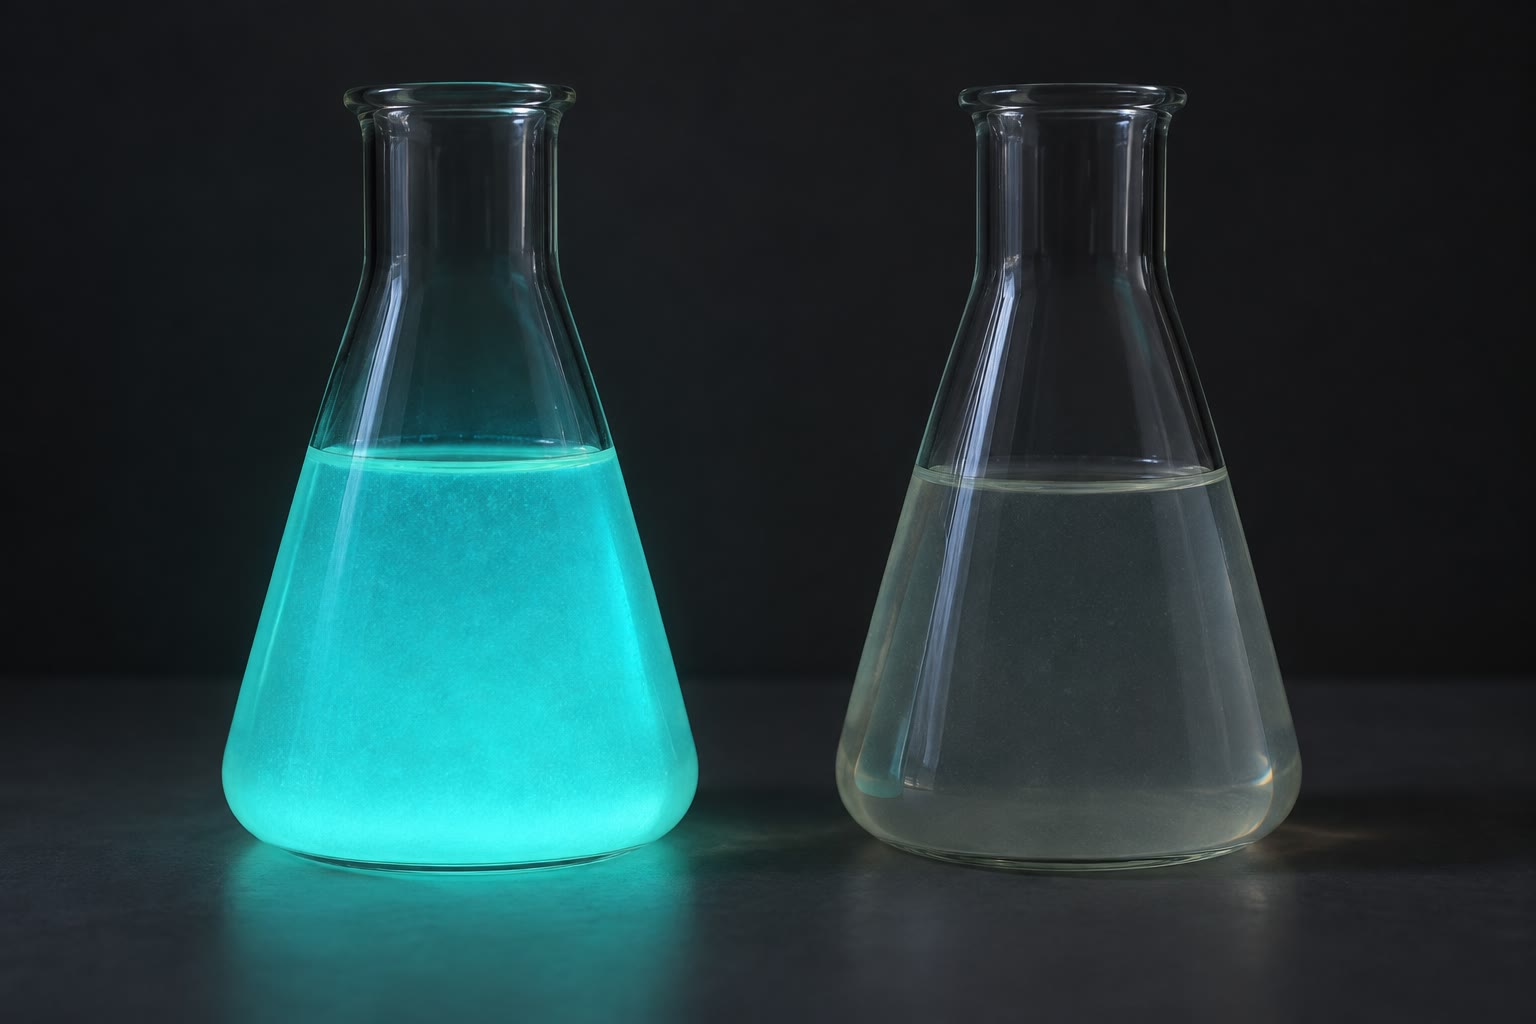
\includegraphics[width=0.46\linewidth]{images/book5/ai/b5-12-quorum-glow.jpg}\hspace{0.04\linewidth}
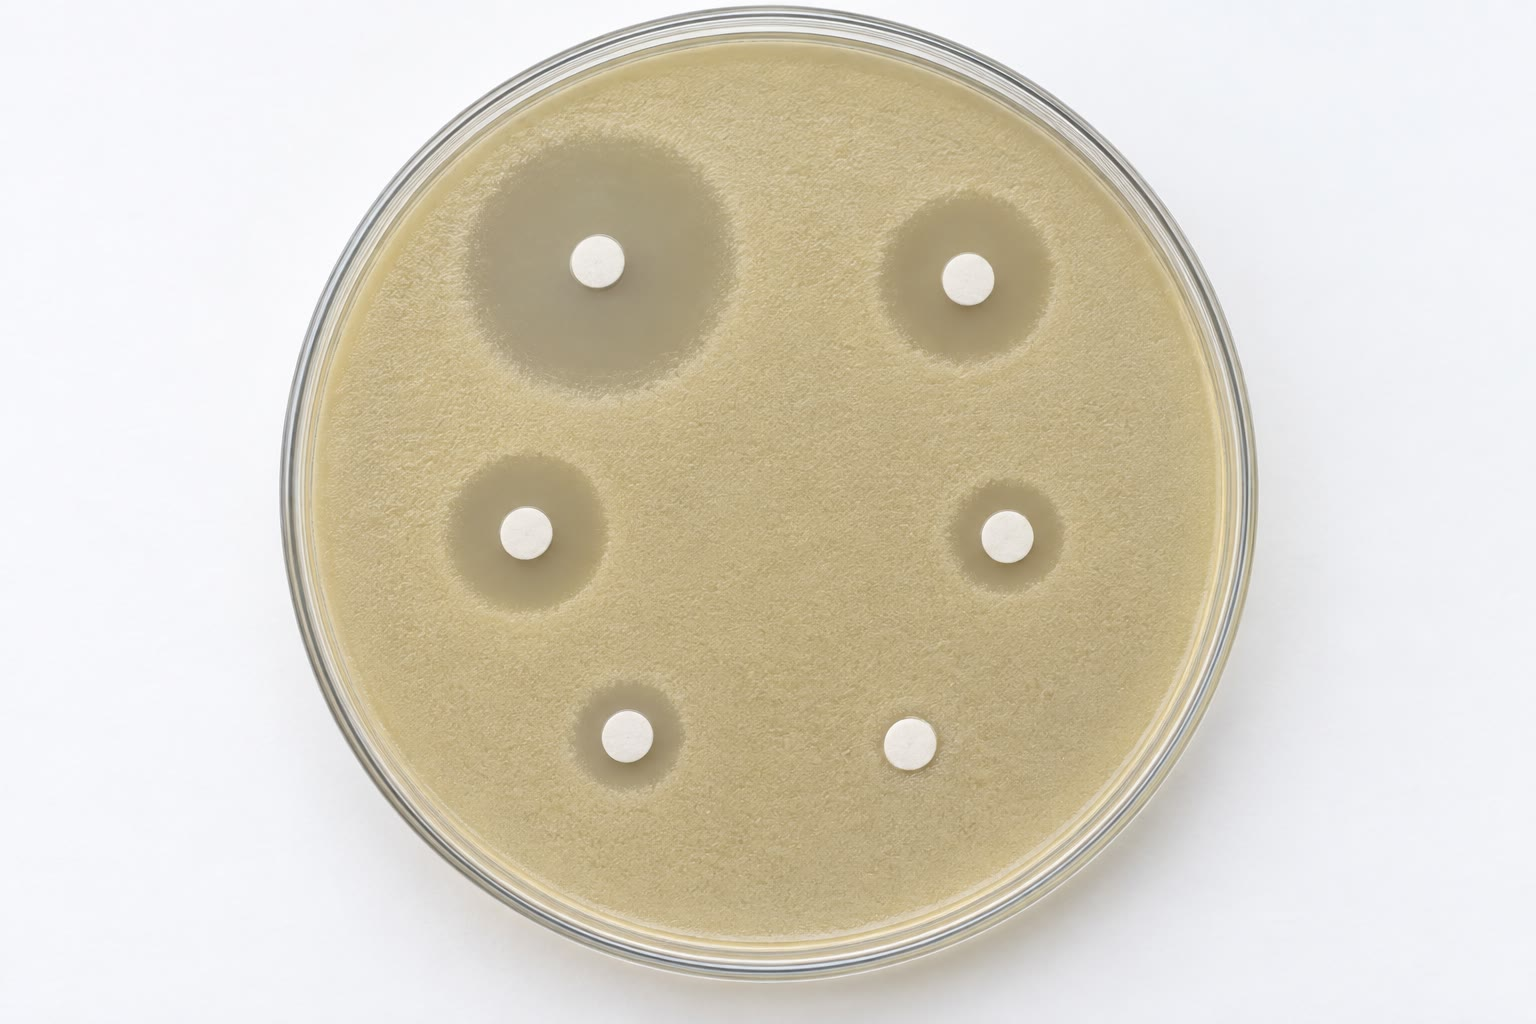
\includegraphics[width=0.46\linewidth]{images/book5/ai/b5-12-antibiotic-disks.jpg}

{\small À esquerda: uma cultura densa de \emph{Vibrio fischeri}
brilhando, ao lado de uma diluída que está escura --- as mesmas células,
acima e abaixo de seu quórum. À direita: um teste de \omterm{met:b3:bacteriology:mic}{difusão em disco};
o diâmetro de cada zona limpa mede a sensibilidade da bactéria ao
\omterm{def:b3:bacteriology:antibiotics}{antibiótico} daquele disco, e o disco sem zona marca uma resistência.}
\end{omfigure}

\section{O tráfego de genes}

\begin{definition}[Transferência horizontal de genes]\label{def:b3:bacteriology:hgt}
\index{transformação}\index{transdução}\index{conjugação}\index{plasmídeo!de resistência}\index{elemento genético móvel}\index{pangenoma}
As bactérias se reproduzem clonalmente, mas trocam genes por três
rotas. A \emph{transformação}: a captação de DNA nu do ambiente por uma
célula competente --- a rota pela qual os pneumococos de Griffith
adquiriram sua cápsula e pela qual Avery mostrou que o princípio
transformante era DNA (1944). A \emph{transdução}: um fago que empacota
um pedaço do DNA do hospedeiro e o injeta no hospedeiro seguinte
(\cref{ch:b3:virology}). A \emph{conjugação}: a transferência de um
\omterm{def:b3:genetic-engineering:tools}{plasmídeo} por um pilus e uma ponte de acasalamento, de um doador que o
carrega a um receptor, demonstrada por Lederberg e Tatum (1946) com
linhagens auxotróficas de \emph{E.~coli} que produziam recombinantes
prototróficos apenas quando misturadas. Os \omterm{def:b3:genetic-engineering:tools}{plasmídeos} conjugativos
carregam seus próprios genes de transferência; muitos carregam também
genes de resistência, muitas vezes agrupados em \emph{integrons} e
ladeados por transpósons, de modo que um único acasalamento pode
transferir resistência a cinco \omterm{def:b3:bacteriology:antibiotics}{antibióticos} ao mesmo tempo, entre
espécies. A consequência é que uma espécie bacteriana tem um genoma
central compartilhado por todas as linhagens e um genoma acessório que
varia --- um \emph{pangenoma}: duas linhagens de \emph{E.~coli} podem
diferir num quinto de seus genes, e as linhagens patogênicas diferem
das inofensivas sobretudo por ilhas adquiridas de genes de virulência.
Os genes do capítulo de mutação do volume do 2.º ano surgem por
mutação; os genes deste, em sua maioria, chegam.
\end{definition}

\begin{omfigure}
\begin{tikzpicture}[every node/.style={font=\scriptsize}, >=stealth]
  % transformation
  \begin{scope}
    \draw[thick, fill=omDef!15] (0,0) ellipse (1.0 and 0.55);
    \draw[omThm, very thick] (-1.9,0.6) .. controls (-1.5,0.8) .. (-1.2,0.5); \draw[->, omThm, thick] (-1.2,0.5) -- (-0.7,0.25);
    \node[below, align=center] at (0,-0.7) {transformação:\\DNA nu captado\\por uma célula competente};
  \end{scope}
  % transduction
  \begin{scope}[xshift=4.6cm]
    \draw[thick, fill=omDef!15] (0,0) ellipse (1.0 and 0.55);
    \draw[thick, fill=omProp!40] (-1.3,1.0) -- (-1.0,1.3) -- (-0.7,1.0) -- (-1.0,0.7) -- cycle; \draw[thick] (-1.0,0.7) -- (-0.9,0.35);
    \draw[omThm, very thick] (-1.1,1.15) -- (-0.9,0.85);
    \node[below, align=center] at (0,-0.7) {transdução:\\um fago carrega um pedaço\\do DNA do último hospedeiro};
  \end{scope}
  % conjugation
  \begin{scope}[xshift=9.6cm]
    \draw[thick, fill=omDef!15] (-1.3,0) ellipse (0.9 and 0.5); \draw[thick, fill=omDef!15] (1.3,0) ellipse (0.9 and 0.5);
    \draw[very thick, omMeth!70!black] (-0.4,0) -- (0.4,0);
    \draw[omThm, very thick] (-1.5,0) circle (0.25); \draw[->, omThm, thick] (-1.25,0) -- (1.0,0);
    \node[below, align=center] at (0,-0.7) {conjugação:\\um plasmídeo cruza\\uma ponte de acasalamento};
  \end{scope}
\end{tikzpicture}

{\small As três rotas da transferência horizontal. Genes de
resistência, de virulência e de metabolismo passam de célula a célula
--- e de espécie a espécie --- mais depressa do que a mutação poderia
fabricá-los.}
\end{omfigure}

\begin{proof}[Evidência]
Robert Koch (1876--1884) estabeleceu que uma bactéria específica causa
uma doença específica: isolou o \emph{Bacillus anthracis} de animais
doentes, cultivou-o em cultura pura em meio sólido (a placa de ágar e a
colônia isolada são invenções de seu laboratório), mostrou que a
cultura reproduzia o antraz em animais sadios e podia ser reisolada
deles --- os postulados que ainda definem um patógeno --- e passou ao
bacilo da tuberculose e ao vibrião do cólera. Alexander Fleming (1928)
notou que um mofo que contaminava uma placa de estafilococos havia
limpado uma zona à sua volta; a substância, a penicilina, foi
purificada e mostrou-se capaz de curar infecções por Florey e Chain
(1940--1941), e em menos de uma década estafilococos resistentes que
carregavam uma enzima destruidora de penicilina já eram comuns nos
hospitais --- um aviso que o próprio Fleming deu em sua palestra do
Nobel.
\end{proof}

\begin{omfigure}
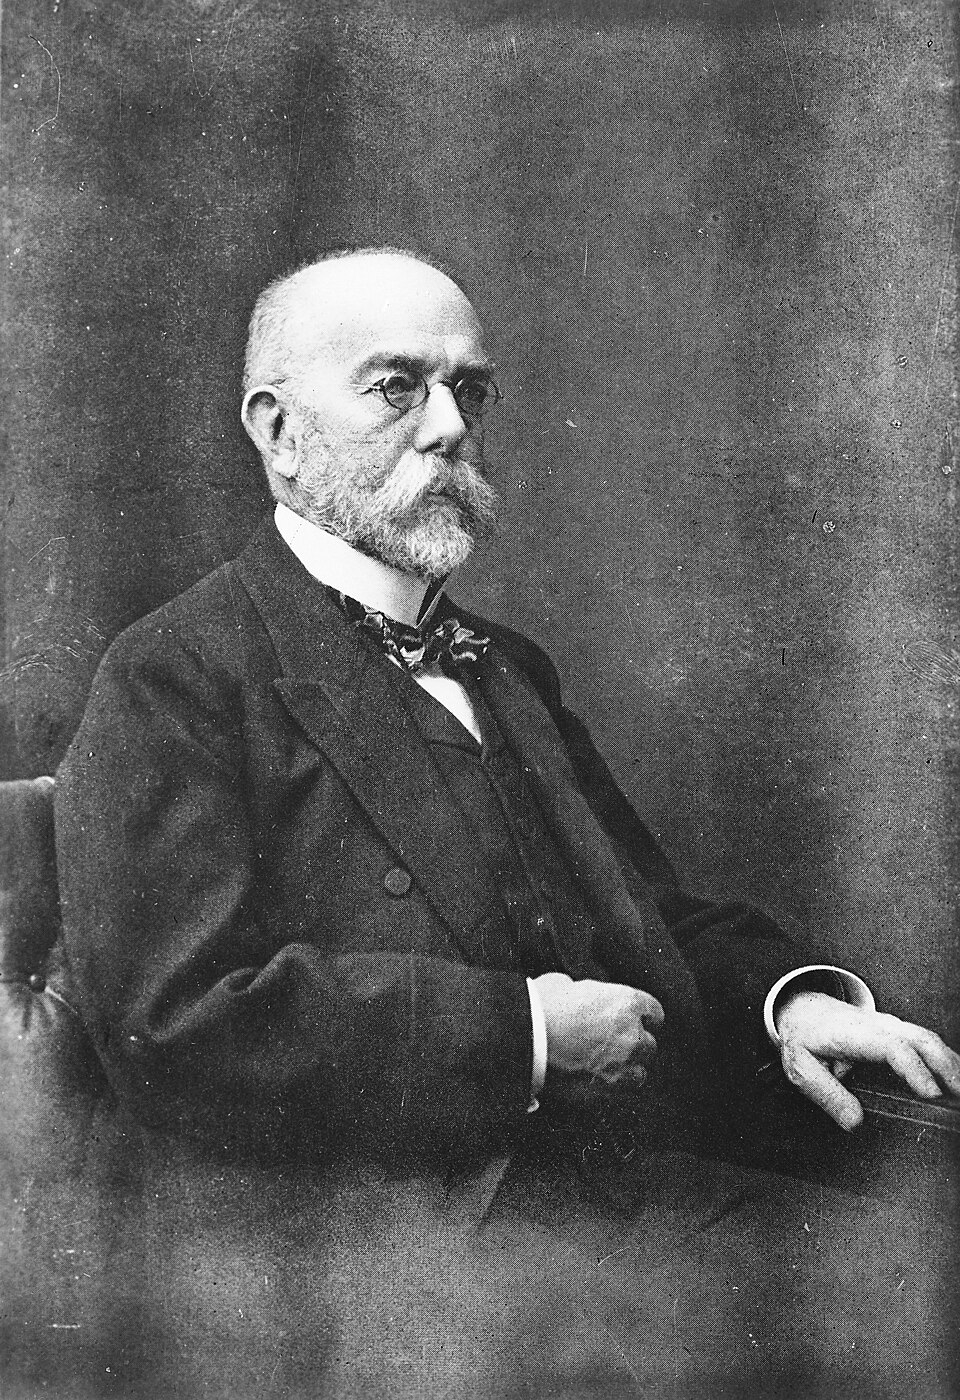
\includegraphics[width=0.30\linewidth]{images/book5/koch.jpg}\hspace{0.04\linewidth}
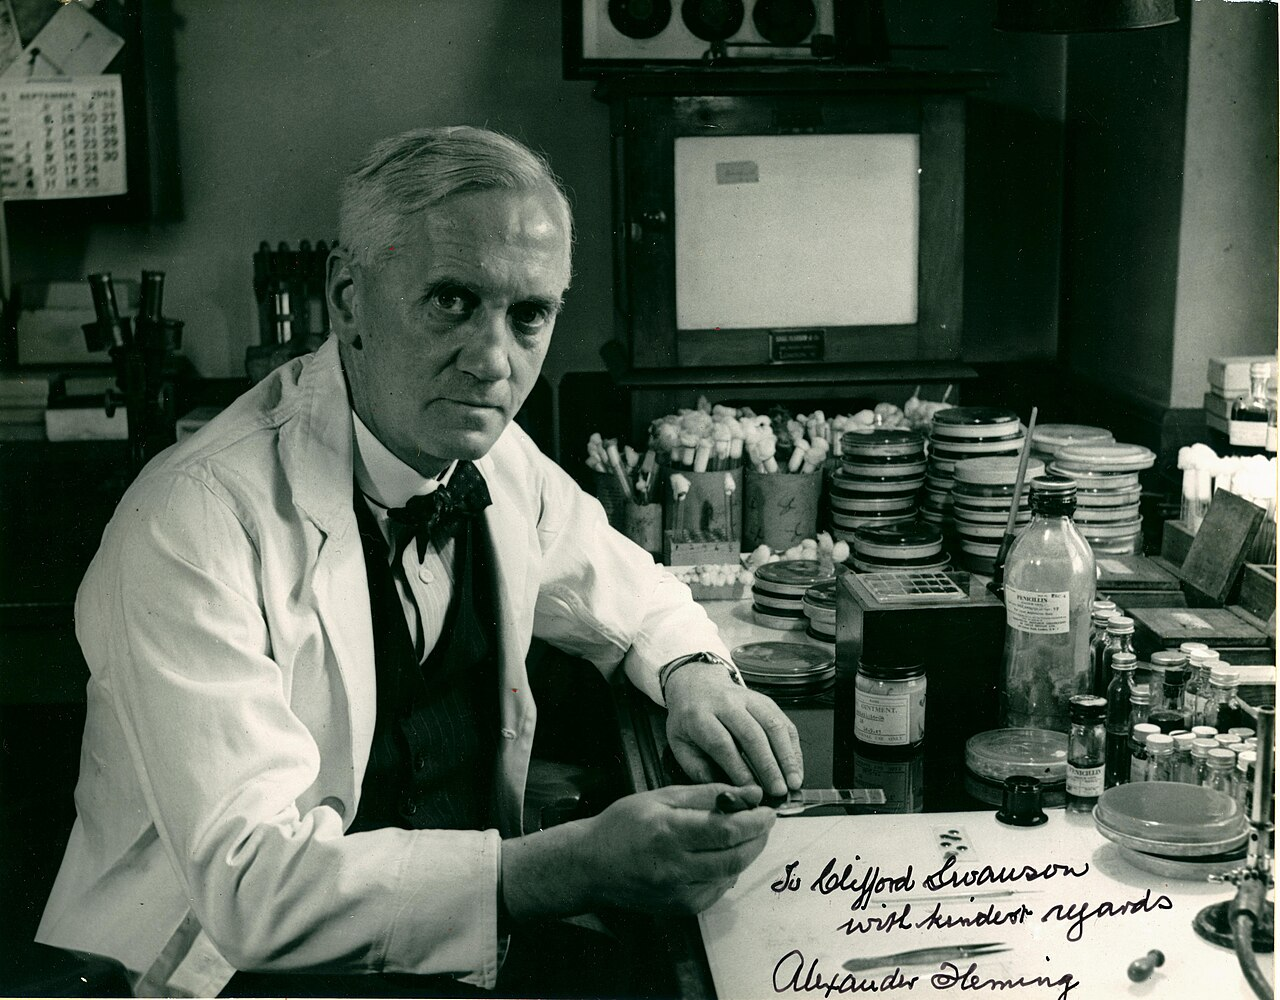
\includegraphics[width=0.56\linewidth]{images/book5/fleming.jpg}

{\small Robert Koch, que provou que bactérias determinadas causam
doenças determinadas e inventou os métodos de cultivá-las (Wellcome
Collection, CC~BY~4.0). À direita: Alexander Fleming em seu laboratório
com placas do mofo cujo produto se tornou a penicilina (arquivo da
Marinha dos EUA, domínio público).}
\end{omfigure}

\section{Antibióticos e resistência}

\begin{definition}[Antibióticos]\label{def:b3:bacteriology:antibiotics}
\index{antibiótico}\index{beta-lactâmico}\index{toxicidade seletiva}\index{concentração inibitória mínima}
Um \emph{antibiótico} é uma molécula que mata bactérias ou detém seu
crescimento em concentrações inofensivas ao hospedeiro, agindo sobre um
alvo que o hospedeiro não tem ou tem de forma diferente --- a
\emph{toxicidade seletiva}. Os alvos são poucos. A parede celular: os
\emph{$\beta$-lactâmicos} (penicilinas, cefalosporinas, carbapenêmicos)
imitam a D-Ala-D-Ala terminal do peptídeo do \omterm{def:b3:bacteriology:envelope}{peptidoglicano} e acilam as
enzimas que fazem suas ligações cruzadas, de modo que a parede em
crescimento fica fraca e a célula estoura sob seu próprio turgor; a
vancomicina liga a própria D-Ala-D-Ala. O ribossomo, cuja forma
bacteriana difere da eucarionte: os aminoglicosídeos (a subunidade
pequena, causando leitura errada), as tetraciclinas (que bloqueiam a
entrada do tRNA), os macrolídeos e o cloranfenicol (o túnel de saída e
a peptidil-transferase da subunidade grande). A DNA-girase e a
topoisomerase~IV: as quinolonas. A RNA-polimerase: a rifampicina. A
síntese de folato, que os animais não fazem: as sulfonamidas e a
trimetoprima. A membrana: as polimixinas, um último recurso. A
\emph{concentração inibitória mínima} (CIM) é a menor concentração de
um fármaco que impede o crescimento visível de uma linhagem; uma
linhagem é chamada resistente quando sua CIM excede a concentração que
o fármaco alcança no paciente.
\end{definition}

\begin{method}[Medir a suscetibilidade]\label{met:b3:bacteriology:mic}
\index{difusão em disco}\index{diluição em caldo}
Dois testes. A \emph{\omterm{met:b3:bacteriology:mic}{diluição em caldo}}: inocule um número fixo de
células (cerca de $5\times 10^{5}$ por mililitro) numa fileira de tubos
ou poços com o \omterm{def:b3:bacteriology:antibiotics}{antibiótico} em passos de duas vezes, incube por uma
noite e leia o primeiro poço limpo: aquela concentração é a CIM. A
\emph{\omterm{met:b3:bacteriology:mic}{difusão em disco}}: espalhe a linhagem numa placa de ágar, ponha
discos de papel carregados com quantidades conhecidas de vários
\omterm{def:b3:bacteriology:antibiotics}{antibióticos} e incube; o fármaco se difunde para fora, com a
concentração caindo com a distância, e o crescimento é inibido até o
raio em que a concentração iguala a CIM, de modo que o diâmetro da zona
limpa --- lido em tabelas calibradas --- dá a suscetibilidade a cada
disco numa só placa. Os dois testes levam um dia; sequenciar o genoma
em busca de genes e mutações de resistência conhecidos leva o mesmo dia
e está começando a substituí-los.
\end{method}

\begin{definition}[Resistência]\label{def:b3:bacteriology:resistance}
\index{resistência a antibióticos}\index{beta-lactamase}\index{bomba de efluxo}\index{MRSA}
Uma bactéria resiste a um \omterm{def:b3:bacteriology:antibiotics}{antibiótico} por um de cinco meios. Ela
destrói o fármaco: as \emph{$\beta$-lactamases} hidrolisam o anel
$\beta$-lactâmico, e as variantes de espectro estendido e as
carbapenemases hoje destroem até os mais novos. Ela altera o alvo: uma
mutação na proteína ribossômica ou na girase que o fármaco liga, ou,
no MRSA (\emph{Staphylococcus aureus} resistente à meticilina), um gene
adquirido de uma enzima de ligação cruzada que os $\beta$-lactâmicos
não ligam; a resistência à vancomicina troca a D-Ala terminal por
D-lactato, que o fármaco não reconhece. Ela bombeia o fármaco para fora
com \emph{bombas de efluxo}, muitas vezes de especificidade ampla. Ela
impede o fármaco de entrar, perdendo uma porina. Ou ela contorna a
etapa bloqueada com uma enzima alternativa. As mutações de alvo surgem
ao acaso no paciente a taxas de $10^{-8}$ a $10^{-6}$ por divisão e são
selecionadas durante o tratamento; as enzimas e as bombas são, em sua
maioria, adquiridas em \omterm{def:b3:genetic-engineering:tools}{plasmídeos} do vasto reservatório de bactérias do
solo e do intestino, no qual evoluíram por eras contra os \omterm{def:b3:bacteriology:antibiotics}{antibióticos}
que fungos e outras bactérias produzem. As persistentes --- células
dormentes que sobrevivem a um fármaco sem serem geneticamente
resistentes --- explicam as recaídas depois de tratamentos que
deveriam ter funcionado.
\end{definition}

\begin{proposition}[Por que a resistência é inevitável e a combinação é a resposta]\label{prop:b3:bacteriology:selection}
\index{resistência!seleção}\index{terapia combinada!antibióticos}
Uma infecção de $10^{9}$ células tratada com um fármaco contra o qual
mutações de resistência surgem a $10^{-8}$ por divisão já contém cerca
de dez células resistentes; o fármaco mata as demais e as dez tomam
conta --- exatamente a aritmética do \cref{ch:b3:cancer-biology}, já
que uma população bacteriana e um \omterm{def:b3:cancer-biology:hallmarks}{tumor} são ambos clones em evolução
sob seleção. Dois fármacos de alvos independentes enfrentam uma célula
duplamente resistente a $10^{-16}$ por divisão, que um bilhão de
células não contém. É por isso que a tuberculose, cujas lesões abrigam
de $10^{8}$ a $10^{9}$ bacilos, é tratada com três ou quatro fármacos
ao mesmo tempo desde os anos 1950, e por que a monoterapia dela
produzia resistência em meses; é também por isso que todo uso de um
\omterm{def:b3:bacteriology:antibiotics}{antibiótico}, num paciente ou num confinamento de gado, seleciona
resistência em algum lugar, e por que o ritmo de \omterm{def:b3:bacteriology:antibiotics}{antibióticos} novos ---
nenhum de classe nova contra \omterm{def:b3:bacteriology:envelope}{Gram-negativas} desde os anos 1960 --- é a
medida contra a qual se contam as perdas. Os remédios são os de
qualquer disputa evolutiva: usar menos, combinar, terminar o
tratamento para que as células parcialmente resistentes não sobrevivam
e se reproduzam, e achar alvos novos.
\end{proposition}

\begin{example}[A janela de seleção de mutantes]\label{ex:b3:bacteriology:window}
Uma linhagem tem CIM de \qty{1}{mg/L}; seus mutantes resistentes de
primeiro passo, presentes a um em $10^{7}$, têm CIM de \qty{8}{mg/L}.
Uma dose que mantenha o fármaco a \qty{4}{mg/L} mata o tipo selvagem e
deixa os mutantes crescerem sem concorrência: a faixa de concentração
entre a CIM do tipo selvagem e a dos mutantes é a \emph{janela de
seleção de mutantes}, e um tratamento que se instale nela cria
resistência. Uma dose acima de \qty{8}{mg/L} mata os dois; uma dose
baixa demais, ou um tratamento interrompido quando o paciente se sente
melhor e o nível do fármaco está caindo pela janela, é como se fabrica
uma população resistente. A mesma lógica fixa os esquemas de tratamento
da tuberculose: seis meses, quatro fármacos, em doses acima da CIM de
todo mutante de um passo.
\end{example}

\begin{omfigure}
\begin{tikzpicture}
\begin{axis}[
  width=0.7\linewidth, height=5.6cm,
  axis x line=bottom, axis y line=left,
  xmin=0, xmax=24, ymin=0.25, ymax=32, ymode=log,
  xlabel={horas após uma dose}, ylabel={fármaco no plasma (mg/L)},
  xlabel style={font=\small, at={(axis description cs:0.5,-0.12)}, anchor=north}, ylabel style={font=\small},
  tick label style={font=\small}, xtick={0,6,12,18,24}, ytick={0.5,1,2,4,8,16}, yticklabels={0.5,1,2,4,8,16},
  clip=false,
]
\fill[omThm!15] (axis cs:0,1) rectangle (axis cs:24,8);
\addplot[very thick, omDef, domain=0:24, samples=60] {16*exp(-0.15*x)};
\addplot[dashed, gray, domain=0:24, samples=2] {1}; \addplot[dashed, gray, domain=0:24, samples=2] {8};
\node[font=\scriptsize, gray, anchor=south west] at (axis cs:0.3,1.05) {CIM do tipo selvagem};
\node[font=\scriptsize, gray, anchor=south east] at (axis cs:23.7,8.4) {CIM do mutante de primeiro passo};
\node[font=\scriptsize, omThm!70!black, anchor=west] at (axis cs:13,3.5) {janela de seleção de mutantes};
\node[font=\scriptsize, omDef, anchor=south west] at (axis cs:2,13) {nível plasmático após uma dose};
\end{axis}
\end{tikzpicture}

{\small A janela de seleção de mutantes. Um nível de fármaco acima da
CIM dos mutantes mata tudo; entre as duas CIMs (área sombreada) ele
mata o tipo selvagem e seleciona os mutantes. Uma dose cujo nível caia
pela janela durante horas, ou um tratamento interrompido cedo, cria
resistência.}
\end{omfigure}

\begin{remark}[A maioria das bactérias não é patógena]\label{rem:b3:bacteriology:most}
As bactérias da clínica deste capítulo são uma minoria ínfima. Do
milhão estimado de espécies, algumas centenas causam doença humana; as
demais tocam os ciclos do nitrogênio, do enxofre e do carbono (o volume
do 2.º ano), fixam o nitrogênio de cada leguminosa, digerem a celulose
de cada ruminante e compõem os microbiomas do
\cref{ch:b3:microbiomes}, cuja perda sob tratamento \omterm{def:b3:bacteriology:antibiotics}{antibiótico} é um
custo de cada tratamento. Os próprios \omterm{def:b3:bacteriology:antibiotics}{antibióticos} são moléculas delas
--- armas e sinais evoluídos entre bactérias do solo e fungos muito
antes de haver hospitais ---, e assim são também a maior parte dos
genes de resistência.
\end{remark}

\section{Exercícios}

\begin{exercise}[$\star$]\label{exo:b3:bacteriology:1}
Descreva os envoltórios Gram-positivo e Gram-negativo e explique por
que a \omterm{met:b3:bacteriology:gram}{coloração de Gram} os distingue.
\end{exercise}

\begin{exercise}[$\star$]\label{exo:b3:bacteriology:2}
Uma cultura de $10^{3}$ células por mililitro chega a $10^{9}$ em
\qty{8}{h} de crescimento exponencial. Determine o número de gerações,
o tempo de geração e $\mu$.
\end{exercise}

\begin{exercise}[$\star$]\label{exo:b3:bacteriology:3}
Nomeie as três rotas da transferência horizontal de genes e dê o
experimento clássico que demonstrou cada uma.
\end{exercise}

\begin{exercise}[$\star$]\label{exo:b3:bacteriology:4}
Dê o alvo da penicilina, da estreptomicina, da ciprofloxacina e da
rifampicina, e diga por que cada uma é seletivamente tóxica.
\end{exercise}

\begin{exercise}[$\star\star$]\label{exo:b3:bacteriology:5}
Um quimiostato tem $\mu_{\max} = \qty{0.8}{h^{-1}}$,
$K_{S} =
\qty{0.02}{g/L}$, $S_{0} = \qty{2}{g/L}$, $Y = 0.4$. Calcule
$S^{*}$ e $X^{*}$ em $D = 0.2$, $0.6$ e $0.79$ h$^{-1}$, e a \omterm{thm:b3:bacteriology:monod}{taxa de
diluição} em que começa a lavagem.
\end{exercise}

\begin{exercise}[$\star\star$]\label{exo:b3:bacteriology:6}
Usando a \cref{prop:b3:bacteriology:threshold}, compare a densidade
limiar da \omterm{def:b3:bacteriology:quorum}{percepção de quórum} no órgão de luz de uma lula
($k =
\qty{0.01}{h^{-1}}$) e em água do mar corrente
($k = \qty{10}{h^{-1}}$), com $p = 100$ moléculas por célula por hora e
$A_{\text{thr}} =
\qty{10}{nmol/L}$ ($6\times 10^{12}$ moléculas por
litro).
\end{exercise}

\begin{exercise}[$\star\star$]\label{exo:b3:bacteriology:7}
Uma placa de \omterm{met:b3:bacteriology:mic}{difusão em disco} mostra zonas de $25$, $12$ e
\qty{0}{mm} para três fármacos. Interprete cada uma e explique por que
um diâmetro de zona pode ser convertido numa CIM.
\end{exercise}

\begin{exercise}[$\star\star$]\label{exo:b3:bacteriology:8}
Explique como um único evento de \omterm{def:b3:bacteriology:hgt}{conjugação} pode tornar uma
\emph{Klebsiella} sensível resistente a cinco \omterm{def:b3:bacteriology:antibiotics}{antibióticos}, e por que
os genes de resistência são tantas vezes encontrados juntos em
\omterm{def:b3:genetic-engineering:tools}{plasmídeos}.
\end{exercise}

\begin{exercise}[$\star\star$]\label{exo:b3:bacteriology:9}
Um paciente tem $10^{9}$ bactérias e toma um fármaco contra o qual a
resistência surge a $10^{-7}$ por divisão. Calcule as células
resistentes esperadas no início; depois, com dois fármacos
independentes. Por que as persistentes são um problema diferente?
\end{exercise}

\begin{exercise}[$\star\star\star$]\label{exo:b3:bacteriology:10}
Mostre que o estado estacionário do quimiostato é estável: perturbe $X$
ligeiramente acima de $X^{*}$ e acompanhe os sinais de
$\mathrm{d}S/\mathrm{d}t$ e $\mathrm{d}X/\mathrm{d}t$. Depois explique
por que duas espécies que competem por um nutriente num quimiostato não
podem coexistir no estado estacionário, e qual delas vence a um dado
$D$.
\end{exercise}

\begin{exercise}[$\star\star\star$]\label{exo:b3:bacteriology:11}
O \omterm{def:b3:bacteriology:quorum}{autoindutor} induz sua própria sintase. Modifique o modelo da
\cref{prop:b3:bacteriology:threshold} de modo que $p$ salte de $p_{0}$
para $p_{1} \gg p_{0}$ quando $A > A_{\text{thr}}$, e mostre que o
sistema pode ter dois estados estáveis ao longo de uma faixa de
densidades (histerese): uma população que já ligou continua ligada numa
densidade em que uma população ingênua estaria desligada. Qual é a
utilidade biológica disso?
\end{exercise}

\begin{exercise}[$\star\star\star$]\label{exo:b3:bacteriology:12}
Explique a janela de seleção de mutantes e use-a para argumentar a
favor ou contra cada uma destas opções: (a) doses altas em tratamentos
curtos; (b) doses baixas em tratamentos longos; (c) parar quando os
sintomas cedem; (d) \omterm{thm:b3:cancer-biology:goldie-coldman}{terapia combinada}.
\end{exercise}

\section{Problema: um quimiostato e uma clínica}

\begin{problem}[{Problema de fim de semana --- uma cultura crescida num
frasco e mantida num quimiostato, uma bactéria luminosa contada até seu
quórum, e uma infecção tratada contra a aritmética da resistência,
terminando nas células do quimiostato, na densidade em que a luz se
acende e nas chances de um tratamento de dois fármacos encontrar uma
célula resistente}]
\label{pb:b3:bacteriology:1}
Dados: \emph{E.~coli} a \qty{37}{\celsius}, $T = \qty{20}{min}$; uma
célula pesa \qty{1}{pg}. Quimiostato: $V = \qty{1}{L}$,
$F = \qty{0.5}{L/h}$, $\mu_{\max} = \qty{1.0}{h^{-1}}$,
$K_{S} = \qty{0.01}{g/L}$, $S_{0} =
\qty{2}{g/L}$ de glicose,
$Y = 0.5$. \emph{Vibrio}: $p = 500$ moléculas de \omterm{def:b3:bacteriology:quorum}{autoindutor} por célula
por hora, $A_{\text{thr}} = 6\times 10^{12}$ moléculas por litro
(\qty{10}{nmol/L}), $k = \qty{0.05}{h^{-1}}$ no órgão de luz. Infecção:
$10^{9}$ células; resistência ao fármaco A a $10^{-8}$ por divisão, ao
fármaco B a $10^{-7}$; CIM do tipo selvagem para A \qty{1}{mg/L},
mutante de primeiro passo \qty{8}{mg/L}; uma dose dá \qty{16}{mg/L},
caindo com meia-vida de \qty{4}{h}.

\medskip
\noindent\textbf{Parte I --- O frasco.}
\begin{enumerate}
  \item Uma célula em \qty{100}{mL} de caldo. Quantas células depois de
        \qty{6}{h} de crescimento exponencial, e que densidade por mL?
  \item O caldo sustenta no máximo $2\times 10^{9}$ células por mL.
        Quando o crescimento para, e qual é a massa de células da
        cultura?
  \item Quanto tempo os descendentes de uma célula levariam para
        alcançar a massa da Terra ($6\times 10^{27}$ g)? Comente.
  \item A \omterm{def:b3:bacteriology:phases}{fase de latência} dura \qty{1}{h} quando células da \omterm{def:b3:bacteriology:phases}{fase
        estacionária} são inoculadas em meio fresco, e quase nada quando
        se usam células em fase exponencial. Explique.
  \item Calcule $\mu$ a partir de $T$. Se o meio for trocado por um
        açúcar em que $T = \qty{60}{min}$, qual é $\mu$, e por qual
        fator cai o número de células depois de \qty{6}{h}?
  \item Uma amostra da cultura estacionária é espalhada numa placa e dá
        $200$ colônias a partir de \qty{0.1}{mL} de uma diluição
        $10^{-6}$. Qual é a contagem de viáveis, e por que ela pode
        diferir de uma contagem ao microscópio?
\end{enumerate}

\medskip
\noindent\textbf{Parte II --- O quimiostato.}
\begin{enumerate}[resume]
  \item Calcule a \omterm{thm:b3:bacteriology:monod}{taxa de diluição} $D$ e o tempo de geração que a
        cultura é forçada a adotar.
  \item Calcule $S^{*}$ e $X^{*}$ (em g/L e em células por mL).
  \item Quantas células deixam o recipiente por hora? Por quantas
        gerações a cultura passa num mês?
  \item A bomba é acelerada para $F = \qty{0.95}{L/h}$. Novos $S^{*}$ e
        $X^{*}$? O que acontece em $F = \qty{1.1}{L/h}$?
  \item Surge um mutante com $\mu_{\max} = \qty{1.2}{h^{-1}}$ e o mesmo
        $K_{S}$. Em $D = 0.5$, de que $S^{*}$ ele precisa, e o que
        acontece com a linhagem original? (Use o
        \cref{exo:b3:bacteriology:10}.)
  \item Um mês de operação são $700$ gerações. Se uma mutação benéfica
        surge a $10^{-9}$ por divisão e o recipiente abriga $10^{12}$
        células, quantas mutações benéficas surgem por geração? O que
        isso diz sobre a evolução num quimiostato?
\end{enumerate}

\medskip
\noindent\textbf{Parte III --- O quórum.}
\begin{enumerate}[resume]
  \item Calcule a densidade celular limiar para a luz no órgão de luz,
        em células por mL.
  \item O órgão de luz contém \qty{1}{\micro L} de bactérias a
        $10^{10}$ por mL. Por qual fator o \omterm{def:b3:bacteriology:quorum}{autoindutor} está acima do
        limiar?
  \item Na água do mar o sinal é levado embora com
        $k = \qty{20}{h^{-1}}$. Densidade limiar? Compare com as
        $10^{2}$ células por mL do mar aberto.
  \item Depois que a lula expele \qty{90}{\%} das bactérias ao
        amanhecer, quanto tempo até que as $10^{9}$ por mL restantes,
        dividindo-se a cada \qty{2}{h}, restaurem $10^{10}$ por mL? A
        luz se apaga nesse meio-tempo?
  \item Cada célula que brilha gasta cerca de \qty{20}{\%} de sua
        energia com luz. Por que uma célula escura é favorecida no mar,
        e não no órgão?
  \item Um patógeno usa o mesmo sistema para adiar suas toxinas até
        estar numeroso. Proponha uma estratégia de fármaco que explore
        isso e diga por que ela poderia selecionar resistência mais
        devagar que um \omterm{def:b3:bacteriology:antibiotics}{antibiótico}.
\end{enumerate}

\medskip
\noindent\textbf{Parte IV --- A clínica.}
\begin{enumerate}[resume]
  \item Número esperado de células resistentes a A no início do
        tratamento; a B; aos dois.
  \item Probabilidade de não existir célula resistente a A; e aos dois.
  \item Depois da dose, quando o nível do fármaco cai a \qty{8}{mg/L} e
        a \qty{1}{mg/L}? Quanto tempo por dose ele passa na janela de
        seleção de mutantes?
  \item Se o fármaco for dado a cada \qty{12}{h}, que fração do tempo o
        nível está na janela, e o que isso prevê ao longo de um
        tratamento de dez dias só com A?
  \item Sugira uma mudança de posologia que mantenha o nível acima de
        \qty{8}{mg/L} o tempo todo (calcule o intervalo ou a dose
        necessária) e enuncie seu custo.
  \item Uma célula em $10^{4}$ é persistente, dormente e intocada por
        qualquer concentração dos dois fármacos. Quantas sobrevivem ao
        tratamento, o que acontece quando o fármaco é retirado, e o que
        isso implica para a duração do tratamento?
  \item Resuma: as células por mL no quimiostato (questão~8), a
        densidade limiar da luz (questão~13) e a probabilidade de o
        tratamento com dois fármacos não encontrar célula resistente
        alguma (questão~20).
\end{enumerate}
\end{problem}
